\section{Introduzione ai circuiti dinamici}
Tutti i circuiti che contengono componenti come
resistori, induttori e condensatori, generatori indipendenti di tensione e corrente ai quali si associa 
una tensione impressa o una corrente impressa vengono detti circuiti lineari tempo invarianti (LTI).

Se vi sono anche bipoli tempo-varianti come interruttori che si chiudono o si aprono, il circuito
si definisce lineare tempo variante (LTV).

Preso un generico circuito, si vuole determinare una tensione o un'intensità di corrente di un generico
bipolo.

\textbf{Strumenti a disposizione:}

\begin{itemize}
\item Equazioni di interconnessione:
\begin{equation} \label{eq:leggi_kirchooff}
\begin{cases}
        \text{LKC} & \forall \text{ nodo } \sum_{k} (\pm) i_k(t) = 0\ \forall\ t \\
        \text{LKT} & \forall \text{ maglia } \sum_{h} (\pm) v_n(t) = 0\ \forall\ t
\end{cases}
\end{equation}

\item Relazioni caratteristiche dei bipoli coerenti con la scelta dei versi delle grandezze (convenzione del generatore o dell'utilizzatore).
\begin{equation}
\begin{cases}
v_R  = R\cdot i \\
v_L  = L\frac{di_L}{dt} \\
i_C  = C\frac{dv_C}{dt} \\
v_e  = e(t)\\
i_j  = j(t) \\
\end{cases}
\end{equation}
\begin{equation*}
\begin{cases}
\text{interruttori in chiusura a t=0: }  {t<0,\ i = 0\ \forall\ v;\ t > 0,\ v = 0\ \forall\ i} \\
\text{interruttori in apertura a t=0: }  {t<0,\ v = 0\ \forall\ i;\ t > 0,\ i = 0\ \forall\ v} 
\end{cases}
\end{equation*}
\end{itemize}

Le equazioni di interconnessione non sono tutte indipendenti ma è sempre possibile
costruire un set di equazioni indipendenti scegliendo \textit{n-1} nodi o \textit{n-l-1} maglie fondamentali,
dove n ed l sono rispettivamente il numero di nodi e lati del grafo connesso.

NOTA: per ogni induttore la potenza assorbita:
$$ P^a(t) = v_l\cdot i_l = L \frac{di_L}{dt}\cdot i_l = \frac{d}{dt} \left[\frac{1}{2}Li_L^2\right] = \frac{dW_m}{dt} $$ 
L' energia immagazzinata nel campo magnetico dell'induttore invece:
$$\Delta W^a(t_1,t_2) = \int_{t_1}^{t_2} P^a(\tau)d\tau = W_m (t_2) - W_m(t_1) $$
Se in un certo istante di tempo l'induttore presenta una certa quantità di energia in Joule [\si{\joule}] quella sarà la massima energia estraibile.

Per ogni condensatore invece potenza ed energia sono così definite:
$$P^a(t) = \frac{d}{dt} W_e;\ W_e(t) = \frac{1}{2} CV_c^2$$
L'energia sarà immagazzinata mediante il campo elettrico.

Si ha quindi un sistema di equazioni circuitali in cui si ha una parte algebrica con le caratteristiche adinamiche, ossia con caratteristiche
non differenziali e non integrali, più una parte differenziale data dai bipoli dinamici come condensatori e induttori.
In letteratura un sistema simile si indica con DAE (Differential Algebric Equation), differente
dalla ODE (Ordinary Differential Equation).

Le tecniche utilizzate in teoria dei circuiti mirano a trasformare una DAE in una ODE, ossia 
formulare le equazioni circuitali come equazioni differenziali ordinarie, per operare questa trasformazione si fa 
riferimento alla dinamica delle sole {variabili di stato}: $i_l(t),\ v_c(t)$

La loro conoscenza permette di esprimere tutte le altre variabili attraverso relazioni algebriche, vengono definite
variabili \textit{slaved}, perché subordinate alle prime.

Per eseguire ciò si richiama una procedura generale per l'analisi di circuiti lineari tempo varianti (LTV).
Questa procedura si basa su un'analisi a intervallo: si partiziona l'asse dei tempi in intervalli in ciascuno dei 
quali esiste un circuito tempo invariante (LTI) equivalente a quello di partenza.

\begin{figure}[h] %tre stati diversi dello stesso circuito
\centering
 \begin{subfigure}{.3\textwidth}
  \centering
  \caption{configurazione generica}
  \begin{circuitikz}
   \draw (0,0) to [R] (1,0);
   \draw (0,0.6) to [L] (1,0.6);
   \draw (0,1.2) to [C] (1,1.2);
   \draw (0,1.8) to [V] (1,1.8);
   \draw (0,2.4) to [I] (1,2.4);
   \draw (0,3) to [closing switch] (1,3);
   \draw (0,3.6) to [opening switch] (1,3.6);
   \draw (-0.3,-0.3) rectangle (1.3,3.9);
  \end{circuitikz}
 \end{subfigure}
 \begin{subfigure}{.3\textwidth}
  \centering
  \caption{$t<0$}
  \begin{circuitikz}
   \draw (0,0) to [R] (1,0);
   \draw (0,0.6) to [L] (1,0.6);
   \draw (0,1.2) to [C] (1,1.2);
   \draw (0,1.8) to [V] (1,1.8);
   \draw (0,2.4) to [I] (1,2.4);
   \draw (0,3) to [open,o-o] (1,3);
   \draw (0,3.6) to [short] (1,3.6);
   \draw (-0.3,-0.3) rectangle (1.3,3.9);
  \end{circuitikz}
 \end{subfigure}
 \begin{subfigure}{.3\textwidth}
  \centering
  \caption{$t>0$}
  \begin{circuitikz}
   \draw (0,0) to [R] (1,0);
   \draw (0,0.6) to [L] (1,0.6);
   \draw (0,1.2) to [C] (1,1.2);
   \draw (0,1.8) to [V] (1,1.8);
   \draw (0,2.4) to [I] (1,2.4);
   \draw (0,3) to [short] (1,3);
   \draw (0,3.6) to [open,o-o] (1,3.6);
   \draw (-0.3,-0.3) rectangle (1.3,3.9);   
  \end{circuitikz}
 \end{subfigure}
\end{figure}

Supponendo che i generatori indipendenti abbiano grandezze \textbf{limitate}, ossia le tensioni impresse $e(t)$ e le correnti impresse $j(t)$,
in questa ipotesi si sa che le variabili di stato sono funzioni \textbf{continue} ossia:
\begin{equation*}
\begin{split}
i_L (0^+) & = i_L(0^-) \\
v_C (0^+) & = v_C(0^-)
\end{split}
\end{equation*}

La soluzione si determina trovando la dinamica delle variabili di stato in ciascun circuito ausiliario, "incollando" le soluzioni utilizzando la proprietà di continuità delle variabili di stato.

Il problema di risolvere circuiti lineari tempo varianti si scompone nel risolvere tanti circuiti lineari tempo invarianti. Una categoria semplice di circuiti tempo invarianti sono i
circuiti lineari del primo ordine (circuiti RC o RL) con un solo elemento dinamico.
\begin{figure}[h] %circuiti RC ed RL equivalenti
\centering
 \begin{subfigure}{.3\textwidth}
  \centering
  \begin{circuitikz}
   \draw (0,0) rectangle (1.6,1.7);
   \draw (0.3,0.3) to [I] (1.3,0.3);
   \draw (0.3,0.9) to [V] (1.3,0.9);
   \draw (0.3,1.5) to [R] (1.3,1.5);
   \draw (1.6,1.5) to [short,i=$i_C$] (2,1.5)
   to [C,v^=$v_C $] (2,0.4) to [short] (1.6,0.4);
  \end{circuitikz}
  \caption{Circuito RC}
 \end{subfigure} 
  \begin{subfigure}{.3\textwidth}
  \centering
  \begin{circuitikz}
   \draw (0,0) rectangle (1.6,1.7);
   \draw (0.3,0.3) to [I] (1.3,0.3);
   \draw (0.3,0.9) to [V] (1.3,0.9);
   \draw (0.3,1.5) to [R] (1.3,1.5);
   \draw (1.6,1.5) to [short,i=$i_L $] (2,1.5)
   to [L,v^=$v_L $] (2,0.4) to [short] (1.6,0.4);
  \end{circuitikz}
  \caption{circuito RL}
 \end{subfigure}
\end{figure}

Un bipolo adinamico lineare e un bipolo dinamico fanno subito pensare all'utilizzo dei teoremi di Thévenin e Norton, permettendo la riduzione del circuito 
adinamico ad un semplice generatore con un resistore equivalente.

Applicando ad esempio la LKT $e_0(t) = R_{th}\cdot C \frac{dV_C}{dt} + V_C$ si ha l'equazione di stato
del circuito e supponendo di conoscere $V_C(t=0) = V_0 $ allora la soluzione dell'equazione è:
$$V_C(t) = [V_0-V_{C_p}(0)] e^{-\frac{t}{\tau}} + V_{C_p}(t)$$ dove $\tau = R_{th}\cdot C$ e $V_{C_p}(t)$
è la soluzione a regime. 
 
Dopo un intervallo pari a $4\sim 5\ \tau$ si assume il processo di carica o scarica terminato.

Per il circuito RL 
$$I_L(t) = [I_0-I_{L_p}(0)]e^{-\frac{t}{\tau}} + I_{L_p}(t)$$ 
con $\tau = \frac{L}{R_{th}},\ I_0 = I_L (t=0)$

Osservazione: la soluzione generale del circuito RC, ossia la dinamica di $V_c(t)$ può essere espressa 
come la somma di due termini $V_{C_{tr}}(t)$ e $V_{C_p}(t)$, il primo transitorio, che tende a svanire se 
si attende un tempo sufficiente lungo, porta con se la \textit{memoria} dello stato iniziale, memoria che 
viene
persa quando $t>4\sim5\ \tau$, ammesso che $\tau$ sia positiva; esistono infatti alcune combinazioni di 
elementi circuitali che si comportano come un resistore negativo.

Il secondo termine è quello di regime permanente, che ovviamente non ha memoria dello stato iniziale ma 
dipende solo dalla nuova configurazione
del circuito (termine forzato).

La decomposizione in regime transitorio e permanente è una decomposizione generale che vale per qualsiasi circuito, a patto di complicare opportunamente la matematica.

Si parla quindi di evoluzione libera ed evoluzione forzata 
$$\begin{cases}
e_0(t) = R_{th}C\frac{dV_c}{dt} + V_C \\
V_c(0) = V_0
\end{cases}$$
si scompone in:

Evoluzione libera
$$\begin{cases}
0 &= R_{th}C\frac{dV_c}{dt} + V_C \\ 
V_c(0) &= V_0
\end{cases}$$

Evoluzione forzata
$$\begin{cases}
e_0(t) &= R_{th}C\frac{dV_c}{dt} + V_C \\
V_c(0) &= 0
\end{cases}$$

Trattazione analoga (duale) per il circuito RL

\newpage
\subsection{Circuiti lineari tempo invarianti del II ordine}
Divisi in (RC, RL, RLC), la procedura generale di risoluzione richiede tre step:
\begin{enumerate}
 \item Determinazione delle equazioni di stato
 \item Determinazione delle condizioni iniziali
 \item Soluzione del problema di Cauchy
\end{enumerate}

Esempio:
\begin{figure}[H]
\centering
\begin{circuitikz}
 \draw (0,2) to [V,l_=$E$] (0,0);
 \draw (0,2) to [closing switch=${t=0}$](1,2) 
             to [R,l=$R_1$] (2.5,2)
             to [R,l=$R_2$] (4,2)
             to [L,i=$i_L$,l=$L$] (4,0)
             to [short] (0,0);
 \draw (2.5,2)node[circ,color=red]{} to [C,v=$v_C$,l=$C$] (2.5,0);
\end{circuitikz}
\caption{Esempio di un circuito RLC del secondo ordine}
\end{figure}

La dinamica dello stato per $t<0$ è di facile risoluzione, $i_L(t) = 0$, $v_C(t) = 0$
per $t > 0$ invece si analizza il circuito:

Equazioni di interconnessione: 
LKC nel nodo evidenziato in rosso (tra i due resistori)
\begin{equation*}
\begin{cases}
I_1 &= I_C+i_L \ \qquad \text{LKC}\\
E &= R_1\cdot I_1 + v_C\ \qquad \text{LKT} \\
v_C &= R_2 \cdot i_L + V_L\ \qquad \text{LKT} \\
V_L &= L\frac{di_L}{dt} \\
I_C &= C\frac{dv_C}{dt}
\end{cases}
\end{equation*}
Si ricava $I_1$ dalla seconda e si sostituisce nella prima,
ora si ricavano le variabili di stato ottenendo
$$
\begin{cases}
i_C = \frac{E}{R_2} - \frac{v_C}{R_1} - i_L \\
v_L = v_C - R_2 i_L
\end{cases}
$$
Sostituendo le equazioni caratteristiche dei bipoli dinamici:

$$
\begin{cases}
C\frac{dv_C}{dt} = \frac{E}{R_2} - \frac{v_C}{R_1} - i_L \\
L\frac{di_L}{dt} = v_C - R_2 i_L
\end{cases}
$$

Le condizioni iniziali sono 
$$\begin{cases}
v_C(0^+) = v_C(0^-) = 0\\
i_L(0^+) = i_L(0^-) = 0
\end{cases}
$$
Per risolvere queste equazioni conviene ridurle ad un'equazione del secondo ordine ad una sola incognita,
ad esempio si sostituisce nell'equazione che definisce $i_C$, $v_C$ ricavata dalla equazione di
$v_L$, in questo modo si ha un'unica equazione in cui compaiono le grandezze relative all'induttore.

Si ottiene 
\begin{equation}
LC \frac{d^2i_L}{dt^2} + CR_2\frac{di_L}{dt} = \frac{E}{R_1} - \frac{L}{R_1}\frac{di_L}{dt} - \frac{R_2}{R_1}i_L-i_L
\end{equation}
raccogliendo i termini
$$
\frac{d^2i_L}{dt^2} + \left(\frac{R_2}{L} + \frac{1}{R_1C}\right)\frac{di_L}{dt}+ \left(1 + \frac{R_2}{R_1}\right)\frac{1}{LC} i_L = \frac{E}{R_1}\frac{1}{LC}
$$
%ora raccogli i termini
Controlli da eseguire: controllo dimensionale e positività dei coefficienti altrimenti il circuito non sarebbe dissipativo.

L'integrale generale è scritto come somma dell'integrale dell'omogenea associata e dell'integrale particolare.
Si ottiene il polinomio caratteristico a partire dall'omogenea associata, ossia annullando il forzamento:
\begin{equation}
\lambda^2 + \left(\frac{R_2}{L} + \frac{1}{R_1 C}\right)\lambda + \left(1+\frac{R_2}{R_1}\right)\frac{1}{LC} = 0
\end{equation}
La soluzione del polinomio può essere di tre tipi:

\begin{itemize}
\item Caso 1, radici reali e distinte, solitamente negative in sistemi dissipativi, modi naturali aperiodici 
smorzati
$$
i_{L_0} = K_1 e^{\lambda_1 t} + K_2 e^{\lambda_2 t}
$$
\begin{figure}[H]
\centering
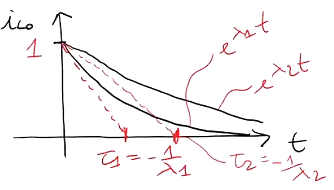
\includegraphics[width=0.4\linewidth]{evoluzione_libera_reali_distinte}
\end{figure}


\item Caso 2, radici reali e coincidenti, caso piuttosto patologico
la radice viene determinata con $-\sigma$ si avrà un modo esponenziale decrescente $e^{-\sigma t} $ con
$\tau = \frac{1}{\sigma}$ e un modo pari a  $t\cdot e^{-\sigma t}$
$$
i_{L_0} = K_1 e^{-\sigma t} + K_2 t\cdot e^{-\sigma t}
$$
\begin{figure}[H]
\centering
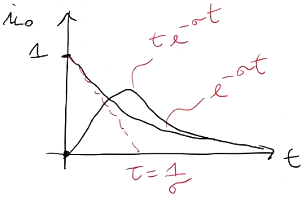
\includegraphics[width = 0.4\linewidth]{evoluzione_libera_reali_coincidenti}
\end{figure}
Vengono detti modi aperiodici smorzati con smorzamento critico.


\item Caso 3, modi periodici smorzati, soluzioni complesse coniugate
$\lambda_{1,2} = -\sigma \pm j\omega_d$, la distanza tra due picchi è pari a $\frac{2\pi}{\omega_d}$
$$i_{L_0}(t) = e^{-\sigma t} [K_1 \cos (\omega_d t) + K_2 \sin(\omega_d t)]$$
\begin{figure}[H]
\centering
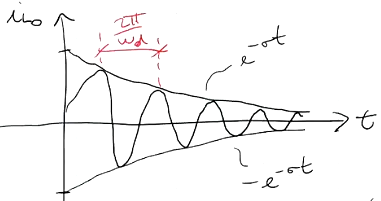
\includegraphics[width=0.4\linewidth]{evoluzione_libera_complesse_coniugate}
\end{figure}
\end{itemize}

Restano da determinare le costanti di integrazione imponendo le condizioni iniziali,
\begin{equation*}
\begin{cases}
i_L(0^+) = i_L(0^-) = \SI{0}{\ampere}\\
\frac{di_L}{dt}(0^+) = \frac{1}{L}[v_C(0^+) - R_2i_L(0^+)] = 0
\end{cases}
\end{equation*}

Supponendo dunque di avere soluzioni $\lambda_1,\ \lambda_2$ reali e distinte e ricordando di aggiungere
il termine a regime $\frac{E}{R_1 + R_2}$ nella determinazione dei coefficienti
$$
\begin{aligned}
i_L(0^+) = 0 & \Rightarrow \\
\frac{di_L}{dt}(0^+) = 0 & \Rightarrow
\end{aligned}
\begin{cases}
K_1+K_2 + \frac{E}{R_1+R_2} = 0 \\
\lambda_1K_1 + \lambda_2K_2 = 0
\end{cases}
$$
La soluzione del sistema permette di ricavare i coefficienti $K_1$ e $K_2$
